\chapter{Analisis}

\section{Analisis Aplikasi Pemantauan Getaran Gedung Berbasis \textit{Wireless Sensor Network}}
Perangkat lunak yang dibangun merupakan sebuah perangkat lunak yang berfungsi untuk memantau getaran gedung menggunakan sensor-sensor yang terhubung dalam sebuah jaringan. Sensor-sensor tersebut akan disebar di sekitar area gedung-gedung dan melakukan sensing terhadap getaran yang dihasilkan oleh gedung tersebut. Kemudian sensor-sensor tersebut mengirimkan hasil \textit{sensing} ke \textit{base station}, berupa besaran sensing dengan satuan gravitasi dari arah X, Y, dan Z. Base-station akan menerima semua hasil \textit{sensing} dan disimpan di komputer dimana \textit{base-station} berada, kemudian diproses untuk memperoleh frekuensi dari getaran pada setiap waktu dan ditampikan ke layar komputer secara visual dan dalam waktu\textit{near realtime}. 

Sensor yang digunakan tidak dibatasi oleh jenis arsitektur WSN yang dapat dipilih. Jenis arsitektur Wireless Sensor Network flat ataupun hirarkikal, dapat digunakan dalam perangkat lunak yang dibangun. Jenis komunikasi \textit{single-hop} ataupun \textit{multi-hop} dapat digunakan pada arsitektur hirakikal seperti yang dibahas pada subbab \ref{arsitektur}.

\subsection{Analisis Arsitektur dan Topologi \textit{Wireless Sensor Network}}
Aplikasi yang dibangun untuk melakukan \textit{sensing} terhadap gedung yang diteliti dan melakukan komunikasi agar data yang ada dapat dikirimkan. Berdasarkan pembahasan tentang arsitektur \textit{Wireless Sensor Network} yang dibahas pada subbab \ref{arsitektur}. Aplikasi ini akan menggunakan arsitektur bertipe flat untuk implementasi. Pemilihan arsitektur flat karena wilayah pengujian gedung yang tidak terlalu luas dan tugas dari setiap node yang disebar memiliki tugas yang sama. Sedangkan berdasarkan pembahasan tentang topologi pada subbab \ref{topologi}, topologi yang diuji untuk membangun aplikasi ini adalah topologi \textit{star} ataupun \textit{linear}. Topologi \textit{linear} dipilih untuk dilakukan pengujian karena topologi \textit{linear} adalah dasar dari komunikasi antar node. Pada topologi \textit{star}, central node akan berfungsi sebagai \textit{sink node} atau dapat dikatakan sebagai \textit{base station} sedangkan node lainnya akan memliki tugas untuk melakukan \textit{sensing} (Gambar~\ref{fig:star_user}).

	\begin{figure}[H] 
		\centering  
		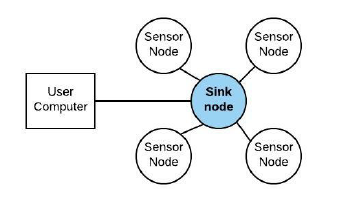
\includegraphics[scale=1]{star_user}  
		\caption[\textit{Wireless Sensor Network} dengan Topologi \textit{Star}]{\textit{Wireless Sensor Network} dengan Topologi \textit{Star}}
		\label{fig:star_user} 
	\end{figure}
	
	\begin{figure}[H] 
		\centering  
		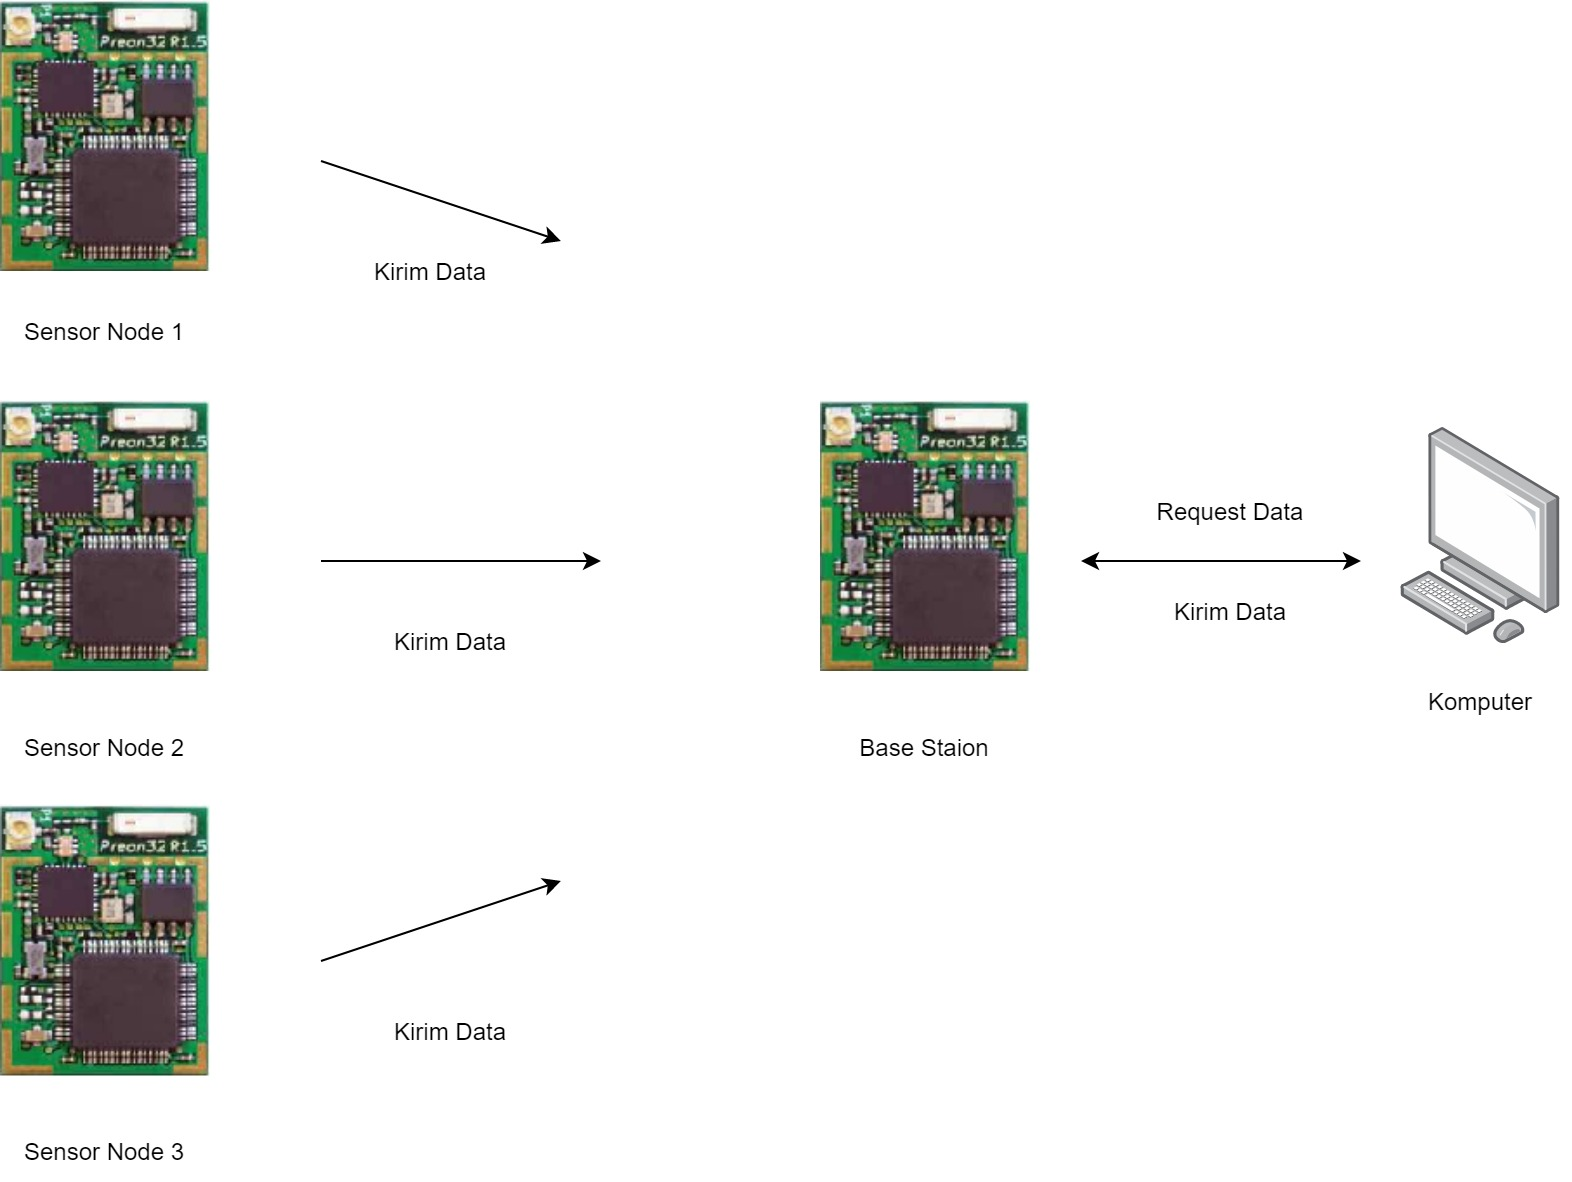
\includegraphics[scale=0.25]{Topologi-WSN}  
		\caption[Arsitektur dan Topologi WSN]{Arsitektur dan Topologi WSN}
		\label{fig:topologi_wsn} 
	\end{figure}

\subsection{Analisis \textit{Accelerometer}}
\textit{Accelerometer} yang akan digunakan dalam penelitian ini adalah \textit{accelerometer} jenis ADXL345 dari sensor node yang berasal dari Preon32 yang ada pada subbab \ref{preonvm}. Jenis \textit{accelerometer} dari Preon32 adalah \textit{three-axis} dan \textit{absolute accelerometer} yang telah dibahas. Hasil \textit{sensing} dari sensor \textit{accelerometer} adalah percepatan dimana dan terdiri dari 3 sumbu yaitu x, y, dan z. Rentang nilai dari percepatan dari sensor ini adalah -255 sampai 255.Nilai percepatan akan dikonversi ke dalam satuan gravitasi (g) dan proses konversi sudah ditangani oleh \textit{class library} yang dimiliki oleh PreonVM yang dimana daftar class librarynya dapat dilihat pada subbab \ref{preon32}.

\subsection{Analisis Fungsi Aplikasi}
\label{fungsi}
Aplikasi yang akan dibangun memiliki fungsi-fungsi utama sebagai berikut:

\begin{enumerate}
	\item Memeriksa status pada setiap node sensor
	
	Fungsi memeriksa status pada setiap node sensor bertujuan untuk memeriksa apakah setiap node aktif atau tidak sebelum melakukan \textit{sensing}. Jika ada sensor node yang statusnya tidak aktif, maka aplikasi akan memberikan informasi berupa adanya node yang tidak aktif dan pengguna dapat melakukan perbaikan atau \textit{maintenance}.
	 
	\item Melakukan sinkronisasi waktu pada setiap node sensor
	
	Fungsi melakukan sinkronisasi waktu pada setiap node sensor diperlukan agar setiap node mengirimkan data hasil \textit{sensing} secara bersamaan atau pada waktu yang sama. Selain itu, \textit{memory} yang ada di setiap node sensor memiliki sifat sementara atau \textit{volatile} (subbab \ref{struktur}). Hal ini menyebabkan adanya kebutuhan untuk menyamakan waktu di setiap node sensor. Karena aplikasi mencatat waktu kapan sensor node itu mati sehingga perlu adanya penyamaan waktu.
	
	\item Mengirimkan perintah yang bertujuan untuk melakukan \textit{sensing}(pengukuran) pada setiap node
	
	Fungsi mengirimkan perintah yang bertujuan untuk melakukan \textit{sensing} pada setiap node digunakan untuk memulai proses \textit{sensing} getaran pada setiap node dengan sensor \textit{accelerometer}. Setiap hasil pengukuran tersebut akan langsung diekstrasi dan dikirimkan ke \textit{base station}.

	
	\item Mengirimkan perintah yang bertujuan untuk memberhentikan \textit{sensing}(pengukuran) pada setiap node
	
	Fungsi mengirimkan perintah yang bertujuan untuk memberhentikan \textit{sensing} pada setiap node digunakan untuk memberhentikan proses \textit{sensing} getaran pada sensor node.
	
	\item Mengubah data hasil \textit{sensing} dari sinyal analog menjadi digital
	
	Fungsi mengubah data hasil sensing dari analog ke digital digunakan untuk mengubah sinyal hasil sensing yang berupa analog menjadi digital (dapat dilihat dengan bentuk angka). Hasil konversi ini pun akan dikirimkan langsung ke \textit{base station} dan akan disimpan ke server atau localhost. Kemudian \textit{base station} akan meneruskan hasilnya ke komputer.
	
	\item Mengirimkan data hasil \textit{sensing} ke \textit{base station}
	
	
	\item Menyimpan data hasil \textit{sensing} yang diterima oleh \textit{base staion}
	
	
	\item Menampilkan data hasil \textit{sensing} yang disimpan oleh \textit{base station}
	
	Fungsi yang terakhir merupakan fungsi yang bertujuan untuk menampilkan hasil \textit{sensing} nya. Fungsi ini dapat dikatakan sebagai fungsi antarmuka dan antarmuka pada aplikasi ini akan menampilkan data hasil \textit{sensing} pada layar komputer pengguna, selain itu juga, antarmuka digunakan untuk melakukan komunikasi antara \textit{base station} dan \textit{node sensor}
\end{enumerate}

\begin{figure}[H] 
		\centering  
		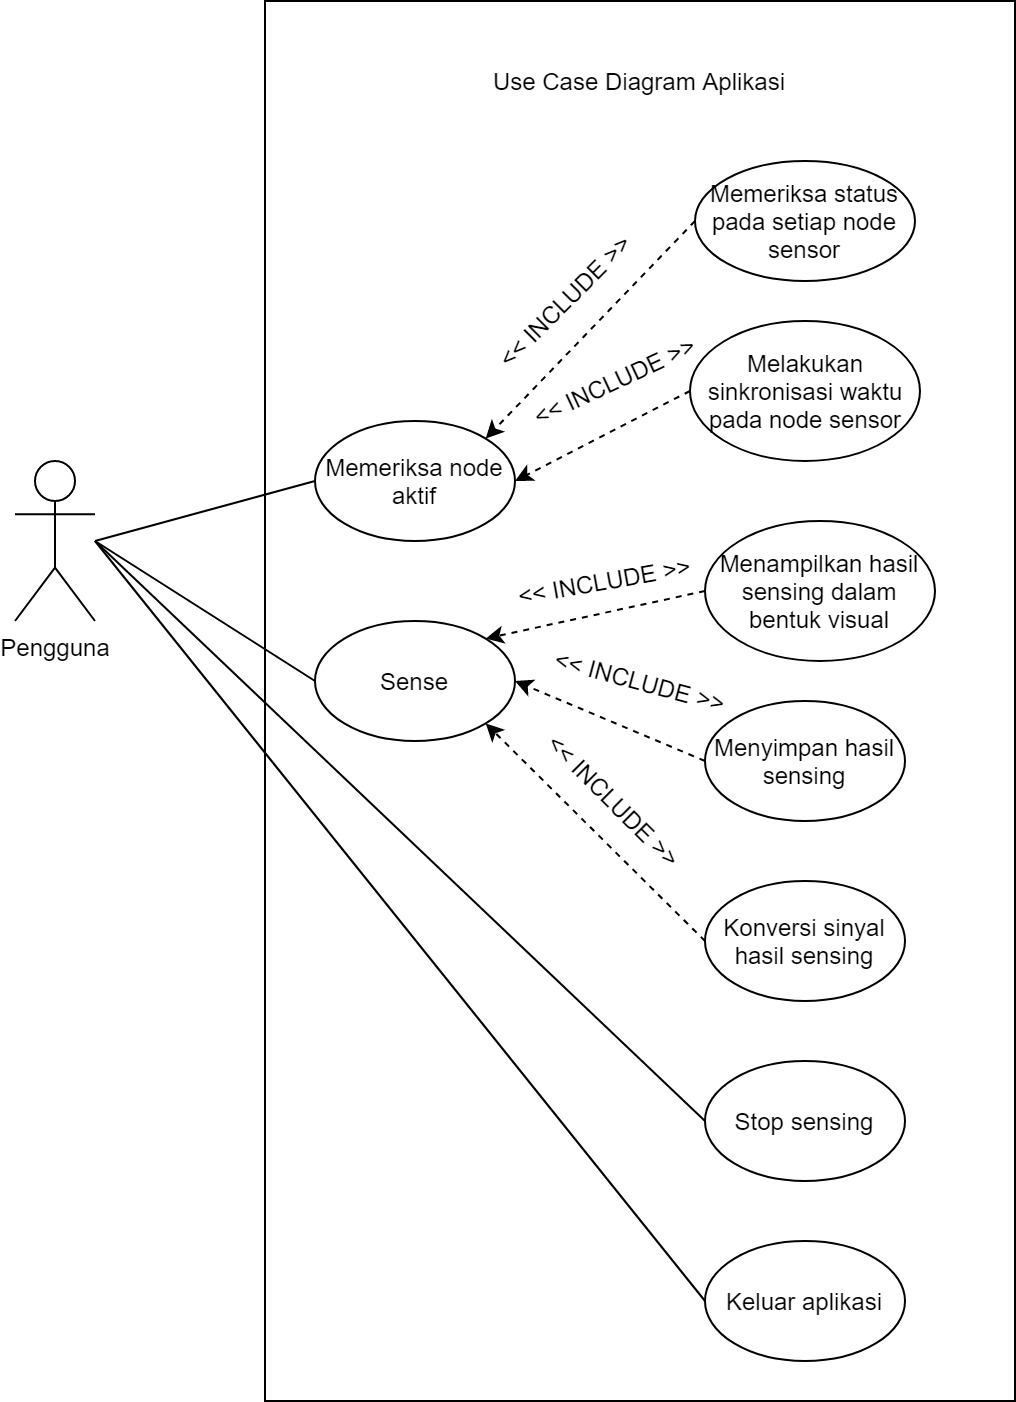
\includegraphics[scale=0.4]{use_case}  
		\caption[Diagram Use Case Aplikasi]{Diagram Use Case Aplikasi}
		\label{fig:use_case} 
\end{figure}


\begin{table}[H]
	\centering
	\caption{Tabel Skenario Memeriksa node aktif}
		\begin{tabular}{|p{.25\textwidth}|p{.70\textwidth}|}
    	\hline
        Nama & Memeriksa node aktif \\ 
        \hline
        Deskripsi & Memeriksa status node sensor aktif atau tidak dan melakukan penyamaan waktu sensor node dengan komputer pengguna\\ 
        \hline
        Aktor & Pengguna\\
		\hline
		Pre-kondisi & Aplikasi baru dibuka oleh pengguna\\
		\hline
        Alur Skenario Utama & \begin{enumerate}
				\item Sistem menjalankan aplikasi.
				\item Pengguna memasukan banyak node yang dipakai.
				\item Sistem menampilkan pilihan fungsi yang dapat digunakan.
				\item Pengguna memilih fungsi "Memeriksa node aktif".
				\item Sistem akan menampilkan \textit{sensor node} dan \textit{base station} yang memiliki status online dan waktu pada setiap \textit{sensor node}.
			\end{enumerate}\\
		\hline
		Pos-kondisi & Aplikasi menampilkan sensor-sensor node yang aktif\\
		\hline
    \end{tabular}
\end{table}



\begin{table}[H]
	\centering
	\caption{Tabel Skenario Memberi perintah sense ke sensor node}
		\begin{tabular}{|p{.25\textwidth}|p{.70\textwidth}|}
    	\hline
        Nama & Memberikan perintah sense  ke sensor node / Sense \\ 
        \hline
        Deskripsi & Memberikan perintah sense ke setiap node sensor dan hasil dari setiap node sensor yang aktif kemudian akan disimpan dan ditampilkan dalam bentuk digital\\ 
        \hline
        Aktor & Pengguna\\
		\hline
		Pre-kondisi & Aplikasi sudah berjalan dan fungsi "Memeriksa node aktif" sudah dijalankan\\
		\hline
        Alur Skenario Utama & \begin{enumerate}
				\item Sistem menampilkan pilihan-pilihan fungsi yang dapat dipilih oleh pengguna.
				\item Pengguna memilih fungsi "Sense".
				\item Sistem akan menampilkan hasil pengukuran (sense) dari setiap node sensor dan menyimpan hasilnya dalam hasil konversi menjadi digital dari setiap node.
			\end{enumerate}\\
		\hline
		Pos-kondisi & Aplikasi melakukan sensing dan menampilkan grafik hasil sensing\\
		\hline
    \end{tabular}
\end{table}



\begin{table}[H]
	\centering
	\caption{Tabel Skenario Stop Sensing}
		\begin{tabular}{|p{.25\textwidth}|p{.70\textwidth}|}
    	\hline
        Nama & Memberikan perintah untuk berhenti melakukan sensing (Stop Sensing) \\ 
        \hline
        Deskripsi & Memberikan perintah berhenti sensing ke setiap node sensor\\ 
        \hline
        Aktor & Pengguna\\
		\hline
		Pre-kondisi & Aplikasi sudah berjalan dan fungsi aplikasi "Sense" dijalankan\\
		\hline
        Alur Skenario Utama & \begin{enumerate}
				\item Sistem menampilkan pilihan-pilihan fungsi yang dapat dipilih oleh pengguna.
				\item Pengguna memilih fungsi "Stop Sensing".
				\item Sistem akan menjalankan fungsi dan menampilkan pesan tunggu sampai fungsi selesai dijalankan.
				\item Semua sensor node akan berhenti melakukan sensing dan tampilan hasil sense akan tertutup dan menampilkan pesan "Sense has stopped".
			\end{enumerate}\\
		\hline
		Pos-kondisi & Aplikasi berhenti melakukan sensing dan grafik sensing tidak diupdate\\
		\hline
    \end{tabular}
\end{table}



\begin{table}[H]
	\centering
	\caption{Tabel Skenario Keluar aplikasi}
		\begin{tabular}{|p{.25\textwidth}|p{.70\textwidth}|}
    	\hline
        Nama & Keluar aplikasi \\ 
        \hline
        Deskripsi & Memberikan perintah keluar aplikasi untuk semua node sensor dan base station\\ 
        \hline
        Aktor & Pengguna\\
		\hline
		Pre-kondisi & Aplikasi sedang berjalan\\
		\hline
        Alur Skenario Utama & \begin{enumerate}
				\item Sistem menampilkan pilihan-pilihan fungsi yang dapat dipilih oleh pengguna.
				\item Pengguna memilih fungsi "Keluar aplikasi".
				\item Sistem menampilkan pesan "aplikasi telah dihentikan".
				\item Aplikasi akan berhenti.
			\end{enumerate}\\
		\hline
		Pos-kondisi & Aplikasi akan tertutup \\
		\hline
    \end{tabular}
\end{table}

\subsection{Analisis Kelas}
\label(kelas)
Pembuatan aplikasi pemantauan getaran gedung menggunakan IDE yaitu Eclipse dan SandBox untuk sensor node Preon32 yaitu salah satu jenis PreonVM yang berasal dari Virtenio. Berdasarkan subbab \ref{fungsi} yang membahas tentang analisis fungsi aplikasi, maka dibuat diagram kelas untuk pembuatan aplikasi ini. Berikut diagram kelas yang dibutuhkan untuk aplikasi ini.

\begin{figure}[H] 
		\centering  
		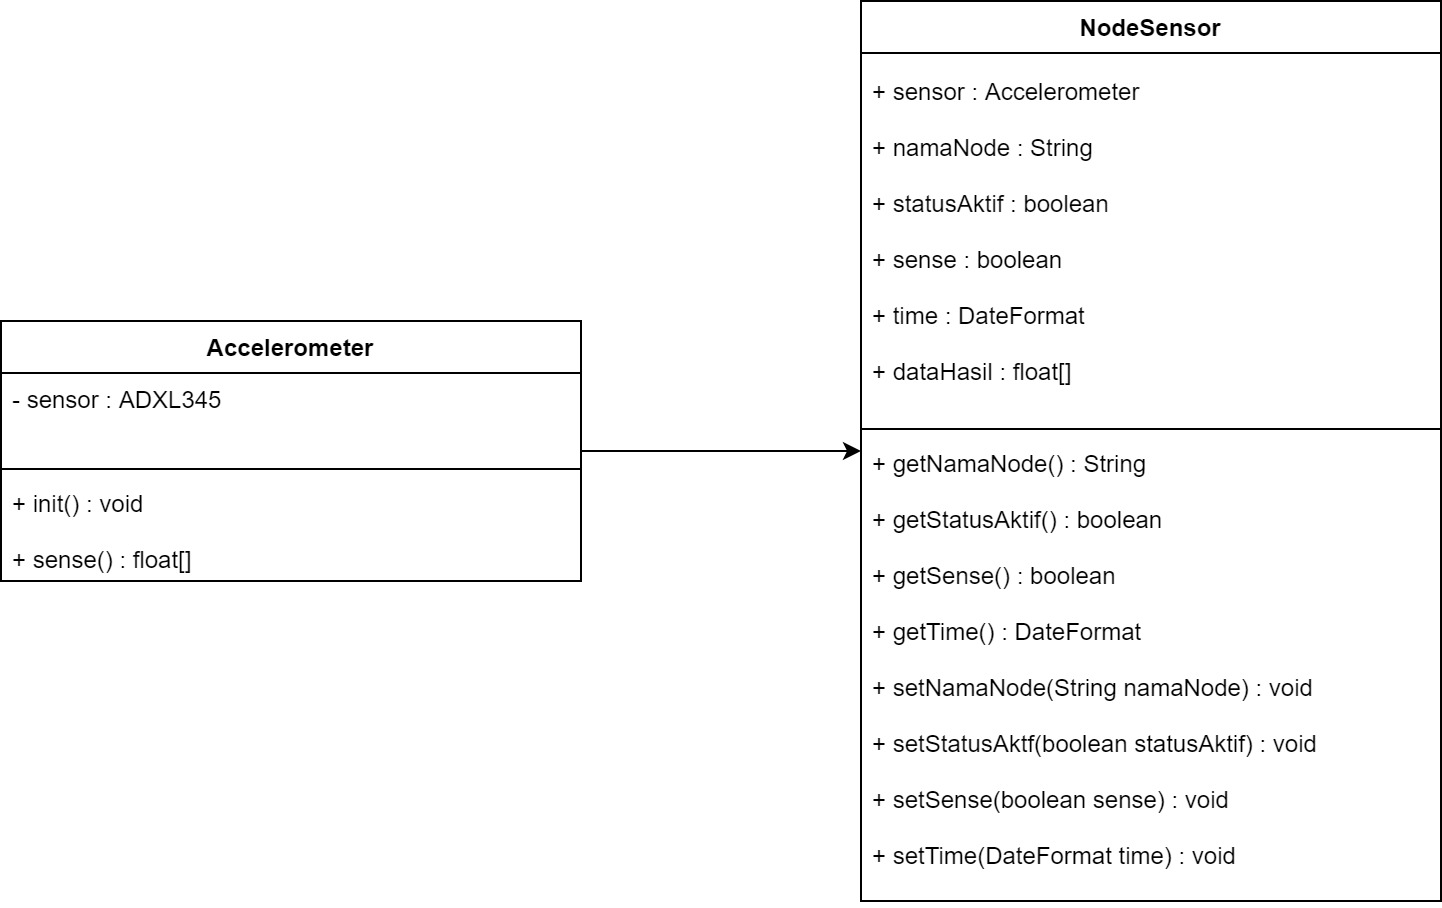
\includegraphics[scale=0.3]{NodeSensor}  
		\caption[Diagram Kelas NodeSensor]{Diagram Kelas NodeSensor}
		\label{fig:user_app} 
\end{figure}

Penjelasan Kelas Accelerometer dan NodeSensor:
\begin{itemize}
	\item Kelas Accelerometer
	 Pada kelas Accelerometer terdapat sebuah atribut yaitu sensor dengan tipe data ADXL345 dimana fungsi atribut ini adalah mempresentasikan jenis sensor yang akan digunakan. Sedangkan pada methodnya terdapat dua method yaitu init() dan sense(). Method init() digunakan untuk menginisialisasi kelas Accelerometer dan method sense() digunakan untuk melakukan sensing (pengukuran).
	 
	 \item Kelas NodeSensor
	 Pada Kelas NodeSensor terdapat beberapa atribut berupa sensor dimana atribut ini akan merujuk ke kelas Accelerometer, kemudian atribut namaNode untuk memberikan identitas terhadap node, statusAktif digunakan untuk memberikan kondisi node sensor sedang aktif atau tidak, atribut sense ada untuk memberikan kondisi apakah node sensor sedang melakukan \textit{sensing}(pengukuran) atau tidak. Atribut time ada untuk mencatat waktu agar node sensor dapat sama ketika melakukan \textit{sensing}. Atribut dataHasil digunakan untuk mencatat hasil pengukuran yang telah dilakukan oleh node sensor. Terdapat juga beberapa method-method untuk kelas NodeSensor berupa \textit{setter} dan \textit{getter} untuk atribut-atribut yang ada pada kelas NodeSensor.
\end{itemize}


\begin{figure}[H] 
		\centering  
		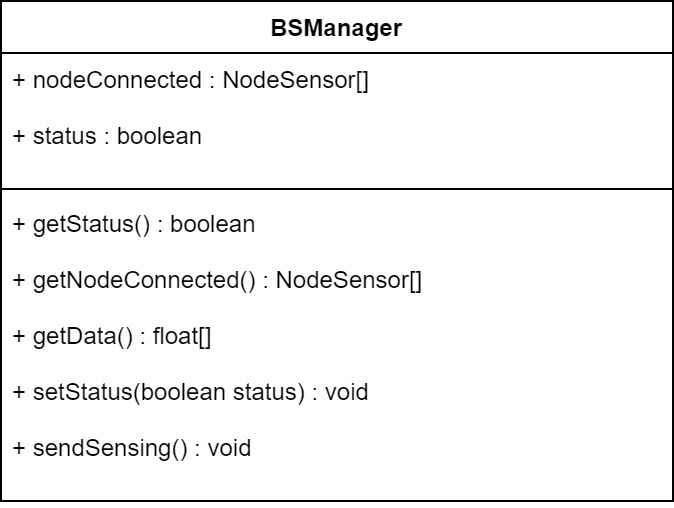
\includegraphics[scale=0.4]{base_station}  
		\caption[Diagram Kelas BaseStation]{Diagram Kelas BaseStation}
		\label{fig:base_station} 
\end{figure}

Penjelasan Kelas BSManager:
\begin{itemize}
	\item Kelas BSManager
	Pada Kelas BaseStation, terdapat dua atribut yaitu nodeConnected dimana ada untuk mengetahui Base Station terhubung ke node yang mana saja kemudian ada atribut status dimana ada untuk mengetahui kondisi Base Station apakah aktif atau tidak. Terdapat beberapa method juga pada kelas BSManager yaitu \textit{setter} dan \textit{getter} untuk atributnya kemudian ada method getData() dimana ada untuk mengambil data hasil \textit{sensing} dari node-node yang terhubung. Method sendSensing() digunakan untuk mengirimkan hasil dari method getData() untuk dikirimkan ke komputer pengguna. 
\end{itemize}

\begin{figure}[H] 
		\centering  
		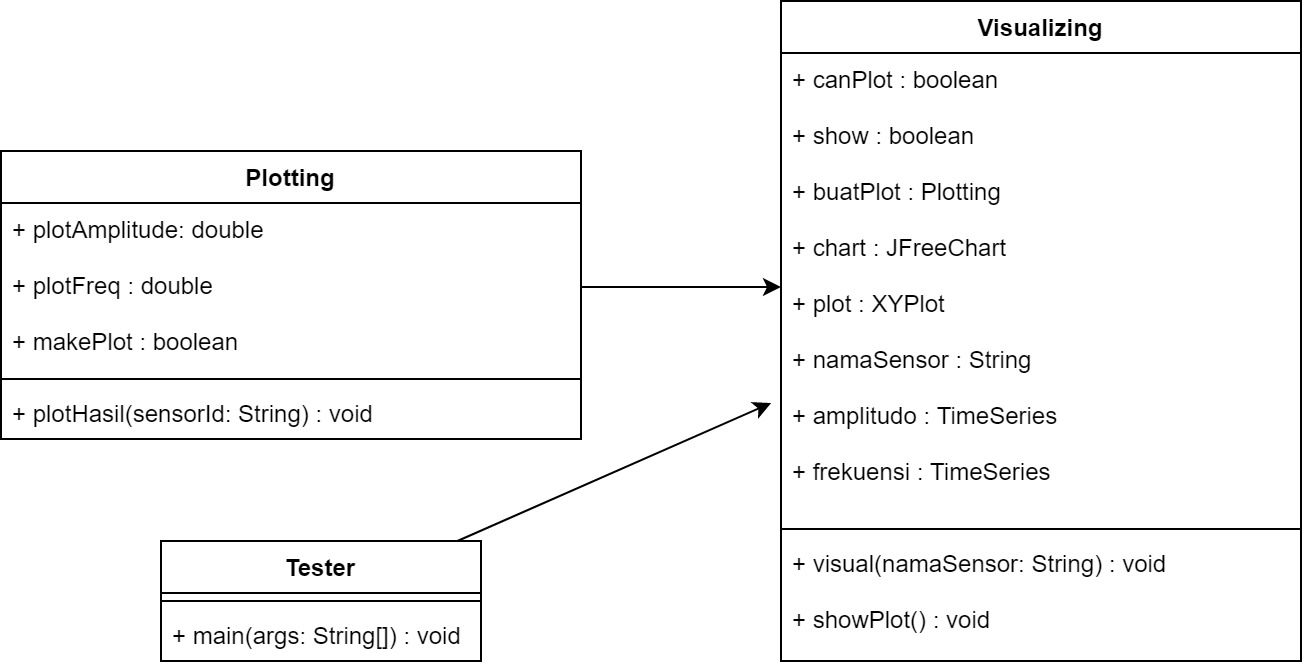
\includegraphics[scale=0.3]{Tester}  
		\caption[Diagram Kelas Tester]{Diagram Kelas Tester}
		\label{fig:use_case} 
\end{figure}

Penjelasan Kelas Plotting, Visualizing dan Tester:
\begin{itemize}
	\item Kelas Plotting
	Pada Kelas Plotting, terdapat tiga atribut yaitu plotAmplitude dimana ada untuk mencatat nilai amplitude dari plot, kemudian plotFreq ada untuk mencatat nilai frequency dari plot sedangkan atribut makePlot ada untuk penanda pembuatan plot. Untuk method terdapat 1 method yaitu plotHasil(sensorId) dimana method digunakan untuk membuat plot pada visualisasi yang sedang berjalan
	
	\item Kelas Visualizing
	Pada Kelas Visualizing, terdapat beberapa atribut yang ada antaranya canPlot digunakan untuk penanda bahwa dapat dilakukan plot atau tidak, kemudian atribut show digunakan untuk penanda apakah sudah ditampilkan atau belum, atribut buatPlot digunakan untuk membuat objek Plotting, atribut chart digunakan untuk membuat objek JFreeChart, atribut plot digunakan untuk mengatur plot yang akan divisualisasikan, atribut namaSensor dibuat untuk menyimpan nama sensor, amplitudo digunakan untuk membuat plot time series dari amplitudo dan atribut frekuensi digunakan untuk membuat plot time series dari frekuensi. Method yang ada pada kelas Visualizing adalah visual(namaSensor), method ini digunakan untuk membuat konstruktor dari kelas Visualizing dan method showPlot() digunakan untuk menampilkan plot pada aplikasi.
	
	\item Kelas Tester
	Pada kelas Tester, terdapat hanya 1 method yaitu main(args: String[]) dimana method ini digunakan untuk menjalankan aplikasi secara keseluruhan.
\end{itemize}

\subsection{Analisis Paket/Pesan}
Hal pertama yang akan dilakukan adalah sensor node akan disebarkan di sekitar bagian gedung, dan melakukan konfigurasi waktu pada setiap node agar waktu mulai sensing dan pengiriman data juga dilakukan bersama. Setelah itu, sensor node akan dinyalakan dan akan dilakukan pengecekan node yang aktif. Cara pengecekan node yang aktif dengan cara mengirimkan pesan yang dikirimkan oleh \textit{base station} ke setiap node. Informasi yang dikirim adalah bahwa node telah aktif. Sistem akan menampilkan pesan bahwa status node sensor ke sekian yang sebelumnya belum aktif, sekarang menjadi aktif. Lalu akan diketahui tujuan data hasil sensing yang akan dikirimkan. 

Ketika pengguna memberikan perintah sensing, maka sensor node akan melakukan pengukuran (sensing) dan melakukan pengambilan data. \textit{Base Station} akan mengirimkan pesan berupa perintah untuk melakukan sensing ke sensor node yang ada. Data-data tersebut merupakan data getaran-getaran yang terjadi pada gedung tersebut, kemudian akan dikirimkan ke \textit{base station}. \textit{Base station} akan menerima data hasil sensing dari sensor node secara terus-menerus kemudian akan mengirimkan hasilnya ke aplikasi dan akan ditampilkan oleh aplikasi tersebut.

Format pesan yang digunakan untuk melakukan komunikasi antara pengguna, \textit{basestation}, dan \textit{sensor node} dengan menambahkan tanda "@" pada awal pesan. Fungsi dari tanda "@" ini adalah untuk menandakan bahwa pesan berasal dari \textit{basestation} dan akan dikirimkan ke \textit{sensor node}. Contohnya jika pengguna ingin menjalankan fitur "\textit{Check Online Node Status}", maka pengguna akan memasukkan angka "1" ke \textit{command line}. Kemudian pesan "1" akan dikirimkan ke \textit{basestation}. Setelah \textit{basestation} menerima kode pesan dari \textit{command line}, \textit{basestation} akan mengirimkan kode pesan "@1" ke setiap sensor node yang terhubung. Kemudian pesan diterima oleh \textit{sensor node}, maka \textit{sensor node} akan menjalankan fungsinya dan mengirimkan pesan hasil fungsi ke \textit{basestation} dengan format ("1 <<sensorId> online <<waktu sekarang>>). 